\documentclass[a4paper,12pt]{article}

\usepackage[utf8]{inputenc}
\usepackage{graphicx}
\graphicspath{{./Bilder/}}
\usepackage[T1]{fontenc}
\usepackage[ngerman]{babel}
\usepackage{hyperref}
\usepackage[a4paper, left=2cm, right=5cm, top=2cm]{geometry}
\renewcommand{\baselinestretch}{1.5}
\usepackage{cite}
\usepackage{bibgerm}
\setcounter{secnumdepth}{4}

\author{Tobias Sigmann}
\title{Seminararbeit: Lorawan}
\date{\today}

\begin{document}
    \maketitle
    \newpage
    \tableofcontents
    \newpage

    \section{Einführung in Lora}
        Lora ist ein Low Power, Wide Area (LPWA) Netzwerkprotokoll und somit sehr gut für batteriebetriebene kabellose Geräte geeignet. Deswegen wir Lora auch of im Internet of Things (IoT) Bereich verwendet.
        Mittels der bidirektionalen Kommunikation ist es möglich Daten und Befehle über weite Strecken zu übertragen. Leider leidet darunter die Geschwindigkeit, sodas sich Lora nicht als WLAN Ersatz eignet.
        Trotzdem können zwischen 0.3 und 50 kbps erreicht werden. In Europa werden 863 MHz bis 870 MHz verwendet. Allerdings variiert der Frequenzbereich für andere Kontinente. Je nach Bedingungen können so bis zu 20km entfernte Endgeräte erkannt und mit diesen kommuniziert werden.
        Es ist sogar möglich den Standort des Gerätes zu bestimmen.
        
        Eine Alternative zu Lora ist Sigfox, hierrauf werde ich nicht weiter eingehen.
        LoRaWAN 1.1
        \newline    
        \cite{WhatIsLoRa}(Optimiert für Batterie Kapazität(Teilnehmer) Reichweite, Kosten
        mehrjährige Batterielaufzeit, kleine Datenmengen, große Reichweite, LPWAN (Low Power WAN)
        
        Kriterien für Lora: Netzwerk Architektur, Reichweite, Batterielaufzeit, Interreferenzrobustheit, Anzahl Konten, Sicherheit, bidirektionale Kommunikation, verschiedene Anwendungsunterstützung
        
        Orientiert für Mobile Adressierbare Endgeräte)
        \newline{}
            \cite{LoraLimit}(
                alternativen: Sigfox, Ingneu, Dash7

                Klassen Kompromiss zwischen Reichweite, Performance(Latzen/ Durchsatz) und Energiebedarf

                Energiesparend durch ADR (Adaptive Daten Rate)
            )
        \newline{}\newline{} Es wird folgen: Was ist lora, wo und wofür wird es benutzt, wie weit kann man senden und wie schnell...
    \section{Aufbau eines Lora-Netzwerk}
        \marginpar{schreib vielleicht noch hinzu das die geräte auch untereinander fergnüpft sein können}
    
        Lora wird auch Deswegen gerne für IoT-Geräte verwendet, weil der Netzwekaufbau ermöglicht die über Lora verwendeten Daten im Internet abzurufen und so ohne weiteres das Gerät mit dem Internet zu verbinden. Um die von den End-Geräten gesendeten LoRa Pakete auf IP/TCP Pakete umzusetzen wird ein Gateway benötigt, das auf der einen Seite LoRa pakete empfängt/sendet und auf der anderen Seite TCP/IP Pakete verwendet.
        Das Gateway implementiert aber keinerlei Logic. Hierzu ist ein Netzwerkserver zuständig der druch die Gateways das Netzwerk kontrolliert und seuert. Gleichzeitig stellt er die verbindung zu einem Applicationsserver her an den er die vondem Gateway empfangenen Daten sendet und von dem auch Daten an die entgeräte, wieder über das Gateway, gesendet werden.
        Diese Architektur wurde gewählt um die laufzeit der End-Gerät, Anzahl der End-Geräte, Qualität des Signals und SIcherheit des Netzwerkes möglichst hoch zu halten.


        \cite{WhatIsLoRa}(Architektur hat größen Einfluss auf Batterie, anz Teilnehmer, qualität, sicherheit,


        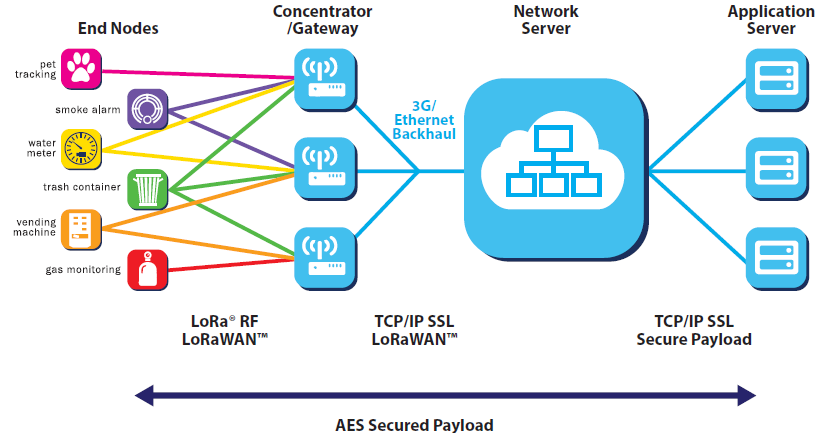
\includegraphics[width=\textwidth]{Netzwerkaufbau}
        
        \subsection{Gateway}
            Das Teilnetz das aus dem Gateway und meheren LoRa-End-Geräten besteht ist Sternförmig aufbau. Jedes End-Gerät kommuniziert diret mit dem Gateway. Diese Atrt der Kommunikation wird auch (Single-Hop-Connection) zu Deutsch (Einfacher-Sprung-verbindung) genannt, da die Gesendeten Daten ohne umwege an das Gateway gesendet werden. Jedes Gatwy ist mit einem Netzwerkserver verbunden.

            Ein Endgeräte kann gleichzeitig an mehren Gateways senden. Der Netzwerkserver ist zuständig die Pakete auf Dublikate zu überprüfen und nur solche nur einmalig an die Appliaktion zu senden.\marginpar{Dabei sind die Endgeräte in Multicast Gruppen unterteilt.}
            Ein weiterer Vorteil ist das kein Handover nötig ist, da alle Gateways fähig sind die Daten des Endgeräts zu verarbeiten bzw. weiterzusenden.
            
            Durch die Sernförmige Architektur des Netzes und die fähigkeit von allen in der Reichweite befindlichen Endgeräte Daten zu empfnagen, muss ein Gatway mit vielen End-Gerätn kommuniziert. 
            Da es nicht möglich ist mit jedem Gerät nacheinander zu kommuniziern, muss dies gelichzeitig geschehen. Hierzu werden adaptive Datenraten und Mehrkanal-Multi-Modem-Transceiver verwendet um eine hohe End-Geräteanzahl zu ermöglichen.
            Außerdem hängt die Anzahl der Teilnehmer davon ab wie geschickt die Kanäle gewählt wurden, welche Datenraten verwendet werden und wie lange gesendet werden muss um die Daten zu senden (man spricht auch von der "Time-On-Air").

            Durch die genannt Eigenschaften der Gateways wird auch eine gute Skallierbarkeit erziehl. Dadurch kann ein neues Gateway die anzahl der Knoten um das 6 bis 8-fach erhöhen. \marginpar{realy?}
            
            \cite{WhatIsLoRa}(
                Meistens wird ein Netzförmiges Netzt aufgebaut. Knoten leiten Nachrichten weiter => größere Reichweite aber kompliziert, erlaubt weniger Teilnehmer und energieaufwändig). 

                Lora Sternförmig => Energie-effizient, Knoten senden direkt an Gateways. Gateways senden an Server, Server muss doppelte Pakete filtern, Sicherheitscheck, ACK über bestes Gateway senden, datenrate anpassen.

                Keine Handover

                Gateway müssen viele Geräte handeln da Stern. erreichen durch (adaptive Datenrate, multi chanel/multi modem transive) mehrere Nachrichten auch verschieden Chanels gleichzeitig empfangen

                Wichtige Faktoren(anz. chanels, datenrate(time on air), paylod länge, Sendehäufigkeit)
            
                Skaliert sehr gut => gemacht für große Nutzerzahlen
                Neues gateway kann Knoten 6-8 x verbessern
                )
            \cite{LoRaSpec}(
                Applikation Server -> Zentraler Server(leitend Pakete weiter) -> Gateway(wandelt lorawan in ip Pakete um) -> Endgerät/Knoten       )
        \subsection{Netzwerkserver}
            Der Netzwekserver ist das "Herzstück" eines jeden Lora-Netzwerkes. Im fallen viele AUfgaben zu. Er kann mit meheren Gatways und meheren Applicationsserver verbunden sein.

            Die wichtigste Aufgabe ist das Steuern des Lora-Teils des Netzwerkes. Der Server verwalted jedes End-Gerät seperat indem es mit ihm den zu verwendendn Kanal aushanelt und die datenrate adaptiv kontrolliert wenn ADR(Adaptiv Data Rate) verwendet wird.
            Weiterhin überprüft er die empfangen Pakete auf ihre Korrektheit und Integrität und filtert Duplikate ,die druch das Empfnagen des gleichen Signales an verschiendne Gatways, verursacht wurden. Dabei ermittelt er auch das Gateway das den besten empfang zu de ENd-Gerät hat und nutzt dieses um Daten an das endgeröt zu senden.
            Es ist nicht immer möglich Daten direkt zu senden. Um die Appliaktion-Server zu endlasten Puffert der Netzwerkserver die Daten und sendet sie zum nächt möglichem Zeitpunkten zu senden.
            Desweiteren muss er die empfnagenen Pakte "bestätegen" und leitet join requests an den joiserver weriter

            Eine weitere sehr Wichtige Ausgabe ist es eine APi für den Applikationsserver bereitzustellen um eine einfache und shnelle kommunikation zu ermöglischen.
            
            \cite{LoRaSpec}( Sicherheit(zähler, ...), leited pakete weiter, filtert pakete, merher gateway via ip verbunden, kontrolliert datenrate, chanäle, adaptiv data rate api.
        \subsection{Applicationsserver}
            Dieser Server ist zuständig den die gesendete NAchrichten zu verarbeiten und gegebenenfals sebst welche an die Endgeräte zu senden.
        \subsection{Join-Server}
            Ein Join-Server wird benötigt um den Beitritt mittels OTAA zu ermöglichen. Der Server kann an mehrere NEtzwerkserver verbunden seinund jeder Netzwerkserver kann mehrer Join server haben.
            Wenn ein Endgerät dem Netzwerk beitreten möchte leited der Netzwerkserver die anfragen an den JoinServer weiter. Diser führt dann die nötige schritte des Beitritts aus wie z.B. ableiten von Schlüsseln.
            Um dies zu tun muss ihm der NwkKey und der AppKey bekannt sein, da diese zum verschlüsseln der NAchichten verwendet werdan aber aus sicherheitsgründen nie über das Netzt gesendet werden.
        \subsection{End-Gerät}
            Endgeräte sind Geräte die Informationen mittels Lora empfangen oder senden. Jedes End-Gerät ist mit einem bestimmten Applikationsserver verbunden.
            

            Jedes Endgerät muss zur korrektion funktion mehere wichtige Informationen Speichern.
            \marginpar{ist das wichtig?}
            \begin{itemize}
                \item DevEUI: Globale endgerätid die eindeutig für jedes endgerät definiert ist. (wie mac eines compueters)
                \item JoinEUI: Globale Adresse des JoinServers an den die anfrage gehen soll. wird nur für OTAA geräte benötigt.
                \item NwkKey und AppKey: Werden verwendet um spätere Schlüssel abzuleiten und die kommunikation während des Joinens abzusichern. Dafür mussen sie sowohl dem Join-Server als acuh dem Endgerät bekannt sein da sie nie übertragen werden.
            \end{itemize}
    \section{LoraWan Funktionsweise}
        Im felgenen Kapittel wird näher auf die funktionsweise von LoRaWAN eingegangen. Spezell, liegt der fokus auf dem Netzwerkebitritt, das verwendete Protokoll und wie die Daten  physikalisch Übertragen werden.
        \cite{LoRaSpec}(
            Geschwindigkeit ist kompromiss zwischen abstand/geschw. die untersch freuenzen bze. geschwindigkeiten beinflussen sich nicht gegeseitig => keine inteferenz
            Die Datenrate ist einstellbar, jedoch wird die Reichweite bei höherer Datenrate gemindert. Ein Vorteil von Lora ist, das die einzelnen Datenraten nicht interferieren und so jedes Endgerät seine eigene Datenrate unabhängig von den anderen Verwenden kann.
            Außerdem wird die Datenrate und die Sendeleistung für jedes Gerät separat gesteuert (ADR, Adaprive Data Rate)
        )
       
        \subsection{Schichtenmodell}
            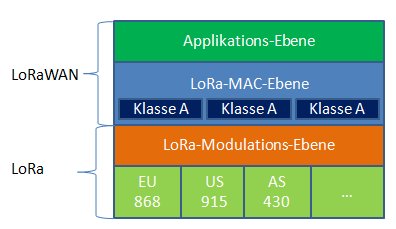
\includegraphics[width=\textwidth]{LoraLayer}

            Das Schichtenmodell lässt sich in zwei Teile unterteilen. Der LoRa Teil ist der unterste und kümmert sich um die Physikalsche übertragung der Pakte und er LoRaWAN teil des Modells ist für die Stuerung des NEtzwerkes, implementierung der LoRaWAN-Klassen und das Überprüfen udn verschlüsseln der Daten zuständig.

            Die Unterste Schicht des LoRa Teils moduliert die verwendeten Frequenzen. In Europa muss das ISM-Band 868 verwendet werden in den Verienigten Staaten wird das BAnd 915 verwendet.

            Die darüberliegende Schicht heißt LoRa Modulation und kümmert sich darum das die Pakete so in die frequenz "moduliert" werden, dass der empfänger diese korrekt und effizent empfangen kann. Meher dazu im kapittel \nameref{sec:Modulation}

            Über der LoRa Modulations schicht liegt die erste LoRaWan schicht, LoRa MAC. Diese sicht ist für die Implementierung der einenel Endgeräteklassen und für das Übertragen der Steuerkomanndos zuständig. Mehr zu den Klassen kann im kapittel \nameref{sec:klassen} und im kapittel \nameref{sec:protokoll} gelesen werden.

            Die oberste schiecht nennt sich Applikationsschicht und ist dafür zuständig die Nutzdaten einer NAchricht passend zu verpacken zu verschlüsseln und zu authentfizieren.

            \cite{WhatIsLoRa}(Application, Lora MAC, MacOptins(Classes), LoraModialtion(Regionales ISB))
        \subsection{Netzwerkbeitritt}
            End-Geräte sind immer bestimmten Netzwerken zugeordnet. Es gibt zwei wege um ein neue End-geräte zu einem bestehenden Netzwerk hinzuzufügen.

            \cite{LoRaSpec}(wei arten OTAA(Over the air activation), ABP(Activation by Personalization)
                    Jedes gerät hat eine vorgegebene DevEUI (wie MAc adresse eines PCs), JoinEUI muss angegeben werden und adressiert den Join server \marginpar{Was macht der? wohin damit?}
                    
            )
            
            
                ABP steht für "Activation by Personalization" und bedeutet Wörtlich übersetzt Aktivierung durch Personalisierung. 

            
            \subsubsection{OTAA}
            \marginpar{umshreiben !!!!!}
            Die sicherste aber auch aufwendigste methode um ein End-Gerät mit einem Netzwerk zu verbinden heißt OTAA (Over-the-Air Activation). Hierbei muss jedes mal wenn einem Netzwerk beigetreten werden soll die Join-Prozedur ausgeführt werden.
            Hierfür müssen folgene 4 Werte Vorgegeben werden. DevEUI, JionEUI , NwkKey, AppKey(Verschlüsselung des join requests).

            
            Als erstes muss das End-Gerät eine join- oder rejoin-Nachricht senden. Die NAchricht besteht aus der JoinEUI, dem DevEUI und einer DevNonce. MIt der DevNonce sollen replayattacs verhindert werden. Sie ist das beim ersten Join request 0 und sollte sich bei jedem Join-Request erhöhen. Außerdem muss sie auch dann noch gespeichert werden wenn kein Strom zur verfügung speht. Falls von dem gelichen endgerät eine Join-Reguest mit einer zu kleinen DevNonce empfagen wir, wird die NAchricht ignoriert und es ist nocht möglich dem Netzwerk beizutreten.

            Die Accept Nachricht besteht aus eier JoinNonce, einem NetzwerkID Net\_ID, einer Geräteadresse DevAddr, einer einstellungsfeld DLSettings , einer angabe wie lange auf eine antwort nach dem senden gerwarted werden muss RxDelay und eriner optionalen liste an Netzwerkparamerter CFList. Die JoinNonce wir außerdem benutz im schlüssel wie AppSKey, ... herzuleiten\marginpar{welche noch, wo beschriebe ich wie?}.
            Für jedes Endgerät wird eine eigene JoinAccept nonce geführt, sie sollte sich nicht wiederholen. Jedes Endgerät merkt sich die letzte JoinNonce und tritt auch nur bei wenn diese großer ist als die letzte empfangene.

            Der NWKSKEY ist für die verschlüsselung der Datenpakete bis zu Gateway zustendig \marginpar{realy? überprüfe die komplette aussage}. Auch dieser Key wird vom Netzwerkserver erzeugt und muss manuell in den code eingetragen werden.
        
            Der letzt Wert heißt APPSKEY und sichert die kommunikation vom End-Gerät zu dem Applikationsserver ab. Der Schlüssel wird genau wie der NWKSKEY vom Netzwerkserver erzeugt und verwalted.
        
            Mehr Infomationen zu den vonkioinsweise der Schlüssel finden Sie in dem Kapittel \nameref{sec:Sicherheit}.


            Wenn der Netzwerkserver den Beitritt des Endgerätes erlaubt sendet er eine Join-Accept nachricht zurück. Das Endgerät erwarted die nachrichten nach JOIN\_ACCEPT\_DELAY1 oder JOIN\_ACCEPT\_DELAY2 nach dem Senden des Request. Sollte die Join-Accept nachricht zu einem andern zeitpunkt gesendet werden, wird diese nicht empfnagen weil das Endgerät nict empfangsbereit ist.
            Die Nachricht enthält einstellungen für das Endgerät sowei die Id des Netzwerkes und die neue Adresse Für das Endgerät. Um replayatacken zu verhindern enthält die nachricht zusätzlich eine JoinNonce. Diese weitd für jedes endgerät seperat geführt und muss größer sein als die zuletzt gesendete.
            
            \subsubsection{ABP}
                Die einfachste Art des Beitritts heist ABP was für "Activation by Personalization" zu deutsch "Aktivierung durch Personalisierung" steht. Hierbei muss lediglich vor inbetribnhme des End-Gerätes 3 Konstanden definiert Werden. Manche Hersteller "brennen" diese 
                drei Werte fest in den chip ein, sodas er nicht geändert werden kann. Flls es nicht möglich ist dem hersteller die gewünschten werte zukommen zu lasse, sind solche End-Geräte nicht für den Beitritt mittels ABP geeignet.
                
                Als erstes muss die DeviceAddress angegeben werden. Diese Adresse existiert nur einmal im Netztwerk und wird verwendet um das Endgerät zu indentifizieren. Die Adrsse wird vom Netzwerkserver erzeugt und muss manuel von dort kopiert werden. \marginpar{gehe ich zu weit?} Die verwendete frequenz entspricht der RX1 bzw RX2 aus dem kapitel \nameref{sec:ClassA}.

                Mit hilfer dieser 3 Werte kann die Join-Request - Join-Accept prozedur übersprungen werden. Daher kann das Gerät direkt einen Loranetz beitreten wenn es angeschalten wird und muss nicht erst alle schlüssel neu ableiten und aushandeln. Allerdings ist diese methode deswegen weniger sicher, da immer die selben schlüssel verwendet werden.

                Nach der verwbindung muss das ResetInd Mac command im FOpt feld gesendet werden gesendet werden solange bis ein ResetConf erhalten wird\marginpar{hab noch nci von mac gesprochen}. NUn ist das Gerät im netzwerk und kann unter der eingestellten Adresse und mit den eigestellten schlüssel arbeiten.
           
                Sobal dem Netzwerk erfolreich beigetreten wurde werden ein die benötigten schlüssel aud dem vorher gesetzetn Werten abgeleited. genauers dazu in kapitel \nameref{sec:Sicherheit}.
        \subsection{Protokoll} \label{sec:protokoll}
            Das LoRaWAN Protokoll ist obtimiert für Batteriebetrieben Endgeräte die draahtlos kommunizieren möchten. Um energieeffizent zu sein setzt LoRa hauptsächlich auf zwei Punkte. Die Modulationstechnick und eine Adaptive Dtanenrate (ADR). Auch die 
            "One-Hop" architektur trät zur energieeffizenz bei. Die Art wie LoRa siganle Moduliert wird in kapittel \nameref{sec:Modulation} besprochen. Um die gannannten Eigenschaften und das Lora Netzwes zu steuern werden sogenannte MAC commands verwendet. 
            Diese werden von Dem Netzwerkserver oder von einem Endgerät gesendet. MAC steht hierbei für "Media Access Protokoll" und bietet die möglichkeit die kommunikation mit den endgeräten, frequenzen, kanäle und vieles mehr zu stuern\marginpar{doppeltgemoppelt}. 
            Da die kommandos nur für den Netzwerkserver und die Endgeräte von bedeutung sind, werden diese nicht an den Applikationsserver gesendet sonder om Netzwerkserver herausgefiltert. Im folgenen wird näher auf die MAC komanndos und die Paketstruktur eingegangen.

            Jedes Pakete besteht aus grundlegend aus 2 Felder (Preamble,  PHYPalyload). \marginpar{erkläre up und downlink} Falls es ich um einen Uplinkpaket handelt wird noch ein CRC code hinzugefügt \marginpar{erkläre crc}  (Preamble,  PHYPalyload, CRC). 
            In diesem fall spricht man von einem implizit Paket oder von dem implezitem modus. Implizit modus bedeute das das es kein payload, codirungsrate und der CRC längenangebe gibt und diese somit eine feste zuvor definierte länge haben. Im expliziten modus werden noch 2 Felder hinzugefügt, 
            PHDR und PHDR\_CRC. SOmit sihet ein explizitest paket folgernermasen aus( Preamble,PHDR, PHDR\_CRC, PHYPalyload). AUch hier gilt, im alle eines Uplinkpaketes wird am ende ein CRC felad angefügt => ( Preamble,PHDR, PHDR\_CRC, PHYPalyload, CRC).
            
            Die Preamble ist dafür gedacht dem Empfänger mitzuteilen das gleich Datengesendet werden. Deswegen wird hier nur ein Signal gesendet das ohne Informationen ist, aber von dem Empfänder wargenommen wird.

            Da Tiele des LoraWAn protokols geschützt sind, finden sich über die PHDR und PHDR\_CRC felder kaum informationan \marginpar{hier das strikt einfügen}. ALlerdings geht herfor das der PHDR die länge des PHYPayloads und die Zieladresse beinhalten sollte. 
            Das PHDR\_CRC Feld wird benutzt um sicherzustellen dass bie empfangenen Werte korekt sind mittels ddes CRC verfahrens \marginpar{erkläre CRC}.
            
            Das CRC Feld 
            
            \cite{LoRaSpec}(
                Mac commands werden benutzt um geräte zu steuern => frequenzen zu ändern, ...
                Application wird diese nie erhalten, läuft zwischen netzwerkserver und lora gerät ab.
                Verschlüsselt hier oder da.
                aufbau: 1byte command, x byte extra data.
                müssen vom empfancher acknolaged werden. Reihenfolge ist zu be<chten. Alle nahrichten in einem farme müssen auch in einem frame ack werden. => Macbuffer ermöglicht dies. Wenn buffer überleuft werden die ältesten ack. \marginpar{(Was passiert mit dem rest?}
                Aloha

                CRC usw wurden fon sender erstellt und eingefügt.
            )
            \cite{LoraClasses}(
                Um energieeffizent zu sein setzt LoRa hauptsächlich auf zwei Punkte. Die Modulationstechnick und eine Adaptive Dtanenrate (ADR)
            )
        \subsection{Übertragungsart}\label{sec:Modulation}
            \cite{LoRaSpec}(
                Knoten können zu jeder Zeit, auf beliebigen Kanälen, beliebig schnell, beliebig lange senden, solange folgende regeln befolgt werden.
                \begin{itemize}
                    
                        \item Channels werden per Pseudozufallszahl geändert
                        \item Sendezeit erfüllt die Regionalen Bestimmungen
                    
                \end{itemize}
            )

            \cite{LoraLimit}(
                Chrip Signal => Zeitliche Änderung in Trägerfrequenz(höhere Frequenz als Datenrate)(positiv chrip/negativ chrip)

                Datensignal wird in Chrip Signal moduliert. Resultierende Signal ist breitbandiger als Datensignal. Maximale Datenrate auch mit Rauschen erreichbar.

                Durch orthogonale "Spread Factor" mehrere Signale auf einem Chanel
            )
            \cite{WhatIsLoRa}(normal FSK, schon sehr efficent. Lora "chirp spread spectrum odulation". Ist wie FSk aber größere Rechiweite, robuster. Stammt aus dem Militär/raumfahrt.Lora als erstes für kommerziellen billigen Einsatz.
            
            Spread spectrum => signale sind Ortohonal für versch. spreizraten, fakto koreliert mit datenrate => verschiedene Datenraten auf einem Kanal
            
            Nähere Geräte sind schneller => höhere Datenrate => kürzee übertrgungsdauer und lassen somit merh zeit für andere, => bessere Batterielaufzeit. Deswegen sidn symetrische up/downlinks nötig.)
            Frequenzhopping, spread spectrum, code-chanels
                \subsubsection{Adaptive Data Rate}
                \cite{LoraLimit}(
                    Datenrate und Funkfrequenz(RF) werde passend zum Abstand angepasst

                    nahe Knoten => hohe Datenrate => kurze Sendezeit => weniger RF-Power
                    kann nach Bedarf geändert werden

                    => immer möglichst schnelle senden => weniger Energie

                )
                \cite{LoraClasses}(crip signal)
    \section{Lora Geräte Klassen} \label{sec:klassen}
        \cite{LoRaSpec}(GGeräte müssen mindestens A können, alle die mehr können werden auch "high class End-Devices" genannt)
        Vieleicht zu klein => in anderes Kapitel stopfen. Bei mehrfacher übertrageung wird nicht erhöht

        Die Endgeräte sind je nach Kommunikationsart/Protokoll Art in drei Klassen (A, B und C) unterteilt. 
        
        Jede Klasse hat 3 counter FCntUP(Pro uplink ++), FCNTDown(pro downlink auser port 0 => mach), AFCntDOwn(port ungleich 0 dann ++)   (nur beschreiben wie diese grob funktionieren) Zähler sollen nich flüchtig sein(Batteriewechseln kein reset)
        bei neuverbinden müssen alle counter auf uf 0 gesetzt werden. counter müssen auf beiden seiten glich gehalten werden(Synchron geführt)
        Wenn nachricht empfagen ist muss der darin enthaltenene counter größer sein als der eigene. 

        die Counter Werte sollen so weit wie möglich nur einam verwendet werden.
        
        )
        \cite{LoraClasses}
        \cite{WhatIsLoRa}(Asynchrone Knoten wegen Batterie => Event/Scheduler gesteuert verwendet ALOHA
        
        Normal Netze müssen sich synchronisieren und Nachrichten abrufen. Lora partiell nicht => laut GSMA 3 bis 5 fach effizienter)
    
        zur besseren Anpassung/ Anpassung an Batterie
        
        EU: 10 Kanäle (8: 250bps bis 5.5kbps) (1: FSK 50kbps) (high rate Lora 114kbps)

        )
        \subsection{Klasse A}\label{sec:ClassA}
            Klasse A zeichnet sich durch sehr geringer Stromverbrauch aus. Die Kommunikation kann bidirektionalen Stadtfinden, allerdings muss die Kommunikation von dem Endgeräte gestartet werden. Das bieted die möglichkeit das das Endgerät, wenn keine Daten gesendet werden müssen, in einen sehr
            sparsamen Schlafmodus wechselt. Um das Endgeräte nicht zum "aufwachen" zwingen zu müssen, wurde auf einen "Hardbeat" oder ähnliches verzichtet. Das Endgerät kann so lange "schlafen" wie es möchte. Dadurch ist die Klasse A auch die potenziell Stromsparende Endgeräteklasse.
            
            Das Endgerät startet die Kommunikation in dem es Daten an das Gateway sendet(uplink). Daraufhin hat das Gateway die Möglichkeit 2 mal Daten zum Endgeräte senden(downlink). Da die Kommunikation asynchron Stadtfinden wartet das Endgeräte bis es beide uplinks empfangen hat.gewünscht.
            
            Um zu ermitteln, wann gesendet werden darf, wird das ALOHA-Protokoll verwendet.
            Da das Gateway nicht immer Daten an die Endgeräte senden kann, muss es diese zwischenspeichern um diese bei der Nächsten Kommunikation zum senden.
            \cite{LoRaSpec}(Es wird zwischen up- / downlink unterschieden)

            \subsubsection{Uplink}

                \cite{LoRaSpec} 
                    (vom Knoten zum Gateway(1..n), Lora radio packet mode, (Preamble, PHDR, PHDR\_CRC, PHYPayload, CRC(cyklische Rendundanz Prüfung))
                 )

            \subsubsection{Downlink}

                \cite{LoRaSpec}
                (
                    radio packet explicit mode, vom Gateway(1) zum Knoten(1), ausgelöst vom Netzwerkserver, auch multikasts möglich, (Preamble, PHDR, PHDR\_CRC, PHYPayload)
                Um Nachricht kurz zu halten kein CRC am ende, nach Reciever\_Delay1 / Reciever\_Delay2 kann empfangen werden (rx1, rx2) 
                
                Fenster müssen lange genug für Preamble auf bleiben=> wenn erkannt wird empfangen wenn nicht fenster weider zu. Es darf nur gesendet werden wenn beide fenster zu sind.
                Es ist auch erlabut andere protokole zu sprechen wenn ncht gesendet oder gehört wird.
                )
                \paragraph{Rx1}
                    \cite{LoRaSpec}(
                        Frequenz abhänig von Uplinkfrequenz, Datenrate abhängig on Uplinkdatenrate, wird nach Reciever\_Delay 1 +/- 20 msec erwarted, Datenrate auch abhänig von Regionalen regeln, Standart: Datenrate = Uplinkdatenrate
                    )
                \paragraph{Rx2}
                    \cite{LoRaSpec}(
                        feste Frequenz/Dtanetnrate, nach Delay2 +/- 20 msec, Frequenz/Datenrate mittels MAC änderbar
                    )
                    \cite{LoRaSpec}(
                        Öffnungslänge muss für Preamble ausreichen, nach RX1 + MIC und autentigitätscheck muss nicht zwingen RX2 geöffnet werden, Sender muss in einem der beiden Fenster stattfinden, Falls Downlink über beide Fenster => feames müsen gleich sein. Knoten dürfen nich während empfangen/ zwischen RX1 und RX2 senden, ender Protokolle dürfen gesprochen werden wenn gesendet werden darf

                        )
        \subsection{Klasse B}
            Die Klasse B bietet bidirektionale Kommunikation mit einer deterministischem downlink Latenz. Um diese latenz zu gewährleisten, muss die Kommunikation Synchron ablaufen. Außerdem muss festgestellt werden, ob das Endgerät bzw das Gateway noch in Reichweite ist. Dies wird mittels einens periodischem "beacon" die zu festgelegten
            Zeitpunkten gesendet werde realisiert.

            Die Latenz ist einstellbar und kann bis zu 128 Sekunden.

            Obwohl das Endgerät durch die periodischen "beacons" nicht "schalfen" kann, ist die Klasse B für den Batteriebetrieb gedacht.
            \cite{LoRaSpec}(wird verwendet wenn mehr bedarf für empfangsfenster ist. Hierzu ist ein synchronsignal nötig=> zu bestimmten zeiten kann damit empfangen werden
                Gateway sended Beacon für synchrinsation. Um daten empfangen zu werden werden empfangsslots => pingslots verwendet, werden periodisch geöffneto und mittels beacon synchronisiert. Normalerweise werde diese schnell geschlossen außer es wird etwas empfagne.
                Gateway dessen beacon benutzt wird, wird nach empfangsqualität ausgewählt. Wenn neuer/unbekanter Beachon von einem anderen GAteway empfangen wird, wird der netzwerkserver benachrichted und dieser entscheidet welcher verwendet wird()passt rozte an).

                Das Netzwerk muss die standart ping-slot periode Datenrate und kanal kennen.

                Um ein gerät auf klasse B zu kommen muss erst von Klasse A gewächselt werden.

                Entgeräte müssen Netzwerkserver über position nformieren. Dies kann über eine leere nachricht passieren oder eine normale(uplink).
                
                Das beacon und die enthaltenen daten werden an die applikation geschiht. Der server kann den beacon auswerten. ziwschen beacon und uplink wird random time verwendet um kolisionen zu verhindern .\marginpar{Nachschuen wie genau das funktioniert}
                änderungen an pingslotperiode .. muss mitgeteilt werden. Hierzu ist klasse A nötig => wechel zu A, wechel zu B.
            
                Beacon wird genutzt um clockdrivt auszugleichen. Wenn kein beacon empfanen wird  => Bacenless mode. Dieser wird bis zu 2 stunden beibehalten. Reines verlassen auf interne Uhr. Wenn beacon empfagne wird, wird zeit zurückgesetzt.
            )
            \subsubsection{Klassenwechsel A nach B}
                \cite{LoRaSpec}(
                    Endgerät fart LoRaWAN layer an. Layer sucht beacon. Mac command DeviceTImeReq um schneller bacon zu bekommen nutzen. Danach wird das ClassB feld auf 1 gesetzt. Bei den geöfneten fenstern wrd der maximal mögliche clockdrift berücksichtigt.
                    Downlink läuft wie bei A ab.


                )
            \subsubsection{Uplink}
                \cite{LoRaSpec}(Wie bei)
            \subsubsection{Downlink}
                \cite{LoRaSpec}(wie bei A, frequenzplan kann sich unterschieden. AUch Multikasts möglich,)
                \paragraph{Singelcast}
                    \cite{LoRaSpec}()
                \paragraph{Multicast}
                    \cite{LoRaSpec}(
                        sepearate Adresse für Multicast
                        Festgelegt durch layer oder manuell für gruppenmulticast
                        Nicht führ MAC geeignet, 
                    )

        \subsection{Klasse C}
            Um eine möglichst geringe/keine Latzen zu erzielen ist die Klasse C gemacht. Dies bedeutet aber auch das der Stromverbrauch am höchsten ist und somit nicht für den Batteriebetrieb geeignet.
            Das Gateway kann immer Daten senden außer wenn das Endgerät gerade Daten sendet. Hier sind Geschwindigkeit von bis zu 50mb möglich.

            Es ist auch möglich während des Betriebes eines Endgerätes die Klasse zu wechseln. Dies wird am häufigste zwischen A und B getan/ ist nur zwischen A und B möglich.
            \cite{LoRaSpec}(
                öffnet RX1 und RX2 fenster wie in Klasse A. Immer wenn  nicht gesendet wird oder RX1 offen ist, ist RX2 offen. Multicast ist auch möglich.
            )
    \section{Sicherheit} \label{sec:Sicherheit}
        Lora bietet die end-to-end Sicherheit an, indem es die Signale zweimal verschlüsselt.

        Die erste Verschlüsselung dient dazu die gesendeten Daten vor eventuellen Mithörern zu verschlüsseln. Die Verschlüsselung geschieht mit einem 128-bit Network-Session-Key.

        Die zweite Verschlüsselung wird bis zur endgültigen Weiterverarbeitung der Daten auf z.B. einen Server verwendet und ist ein 128 bit Application-Session-Key.

        Das zur Verschlüsselung verwendete Protokoll ist AES. Auch zu Authentifizierung und zur Überprüfung der Integrität wir AES verwendet.
        \cite{LoRaSecur}
            \cite{WhatIsLoRa}(Applikationsverschlüsselung(schutz der Daten for mitlesen) Netzwerk(Autentiizierung der Knoten) AFS, Key Exnage IEEE EU164)
            \cite{LoRaSpec}(symetrischer Schlüssel => nur einer benötigt, Sessionkey ist abgeleited von Knoten-rootkey. JoinServer setllt verbindung der Keys her.
            )
    \section{Live-Beispiel}
        wenn vorhanden.

    \section{Fazit}
    \section{Sonstige quellen}
        \url{https://lora-alliance.org/resource-hub}
        QuickStart für ein kleines Projekt: \url{https://www.thethingsnetwork.org/docs/devices/node/quick-start.html#setup-arduino-ide}

        Weitere Infos \url{http://www.multitech.com/documents/publications/marketing-guides/lora_device_dev_guide_orange.pdf}
        \newpage
    \bibliographystyle{geralpha}
    \bibliography{myBib}
    %richtige namen finden
\end{document}